%\documentclass[11pt]{article}
\documentclass{article} % For LaTeX2e
\usepackage{nips13submit_e,times}

\usepackage{graphicx}
\usepackage{epsfig}
\usepackage{caption}
\usepackage{subcaption}
\usepackage{cite}
\usepackage{url}
\usepackage{wrapfig}

\newcommand{\fix}{\marginpar{FIX}}
\newcommand{\new}{\marginpar{NEW}}

\nipsfinaltrue

\begin{document}

\title{Learning connections between layers in deep networks}

\author{
Eugenio Culurciello\thanks{More information on Eugenio Culurciello's laboratory and research can be found here: http://engineering.purdue.edu/elab/. Real time robotic vision systems: http://www.neuflow.org/} \\
Purdue University\\
\texttt{euge@purdue.edu} \\
\And
Jordan Bates \\
Purdue University\\
\texttt{jtbates@purdue.edu}
\AND
Jonghoon Jin \\
Purdue University\\
\texttt{jhjin@purdue.edu}
\AND
Aysegul Dundar \\
Purdue University\\
\texttt{adundar@purdue.edu}
\And
Clement Farabet \\
New York University \\
\texttt{cfarabet@nyu.edu}
}

%\date{\today}

\maketitle

\begin{abstract}
We present the clustering learning technique applied to learning the connection matrix between layers of multi-layer feedforward deep neural networks. We show that networks and connections trained with clustering learning can obtain similar levels of performance as supervised deep network trained to .... 
\end{abstract}


\section{Introduction}

Most scientists and engineers are fascinated by the design of an artificial vision system that can reproduce some of the human visual system capabilities in detecting, categorizing, tracking objects in view. The availability of a real-time synthetic vision system with such capabilities would find use in a large variety of applications, such as: autonomous cars, co-robots helpers, smart appliances, cellular-phones, to name a few.
 
In the recent years the fusion of bio-inspired and neuromorphic vision models with machine learning has dominated the development of artificial vision systems for the categorization of multiple objects in static frames.
Bio-inspired deep networks are computer-vision and computational-neuroscience models of the mammalian visual system implemented in deep neural networks \cite{lecun_gradient-based_1998,hadsell_dimensionality_2006,gregor_structured_2011,riesenhuber_hierarchical_1999,serre_feedforward_2007,serre_neuromorphic_2010}. Most deep network architectures are composed of multiple layers (2, 3 typically), where each layer is composed of: linear two-dimensional filtering, non-linearity, pooling of data, output data normalization \cite{jarrett_what_2009,lecun_convolutional_2010,boureau_theoretical_2010}. 
Recent machine learning research has focused on the task of training such deep networks from the abundant digital data available in the form of image frames and videos. In particular, deep networks need to learn good feature representations for complex visual tasks such as object categorization and tracking of objects in space and time, identifying object presence and absence. These representations usually involve learning the linear filter weight values from labeled and unlabeled input data. Since labeled data is costly and often ridden with human errors \cite{karpathy_lessons_2011, torralba_unbiased_2011, hou_meta-theory_2012}, the recent focus is on learning these features purely from unlabeled input data \cite{olshausen_emergence_1996, hyvarinen_independent_2000, hinton_fast_2006, vincent_extracting_2008, coates_analysis_2011}. These recent methods typically learn multiple layers of deep networks by training several layers of features, one layer at a time, with varying complexity of learning models. Traditional work in deep learning for vision has mostly focused on improving the learning algorithms, and rarely it has shown potential for overcoming some of the limitation of these systems, such as reliance on large sets of labeled data, and real-time operation for embedded systems.

Recent techniques based on unsupervised clustering algorithms are especially promising because they use simple learning methods that quickly converge \cite{coates_analysis_2011}. 
These algorithms are easy to setup and train and are especially suited for robotics research, because less complex knowledge of machine learning is needed, environment-specific data can be collected quickly with a few minutes of video, setup of custom size deep networks is quick and can be adapted to specific tasks. %reword this sentence?
In addition, real-time operation with efficient networks can be obtained with only a few minutes of training and setup, leading to quick and direct experimentation in robotic experiments.

In this paper we present unsupervised clustering algorithms applied to learning the connectivity matrix between layers and filters of deep neural networks for general-purpose vision systems. 
%The main goal of the paper is not to present state-of-art results on a specific dataset. Rather we want to present ways to quickly process video sequences to extract a large portion of information without the need of supervision and heavy learning techniques.
%The goal is also to show that compact video-based unsupervised networks can support at least ten frames-per-second operation on commercial hardware, such as recent laptop computers.

The paper presents the following key innovations: (1) use of clustering learning for learning both filters and connections of deep networks with fully unsupervised techniques (Section \ref{}), (2) the ability of trained network to perform as well as supervised networks trained on still frames, (3) ability to run in real-time?. 



\section{Main idea and contribution}
\label{sec-main}

In this paper we created and tested a model of unsupervised clustering algorithms in deep neural networks. We extend the results obtained in previous work [http://arxiv.org/abs/1301.2820], aimed at learning filters in multi-layer networks, to also learn the connection matrix between layers. 

The connections between layers in a deep neural network are a very important parameter. It has been shown that in many cases random filters perform only slightly worse than fully trained network layers [cite: On Random Weights and Unsupervised Feature Learning, Saxe et all] suggesting that filters (used in the convolutional filtering stage of each layer in a deep network) might not play a dominant role in determining the performance of a deep network.
Rather, the connections between layers and the combination of features are mainly responsible for the recent success of supervised deep convolutional networks [cite: hinton krizevsky 2012 et al]. In these networks the connection between layers is learned from the data using global gradient-descent techniques at large scales.
 
In unsupervised deep networks, one cannot rely on back-propagation techniques to learn the connections between layers. This is because unsupervised networks do not used labeled data, and thus an error signal cannot be computed.
In order to use unlabeled data to train large deep networks, we will need a technique that can derive how to group features from one layer into features of the next layers, and at the same time learn the filters needed by the next layer.
This is the main contribution of this paper, and what makes it unique. A figure that qualitatively explains the main contribution of the paper is Fig. \ref{fig-learnlayers}.

\begin{wrapfigure}{r}{.7\textwidth}
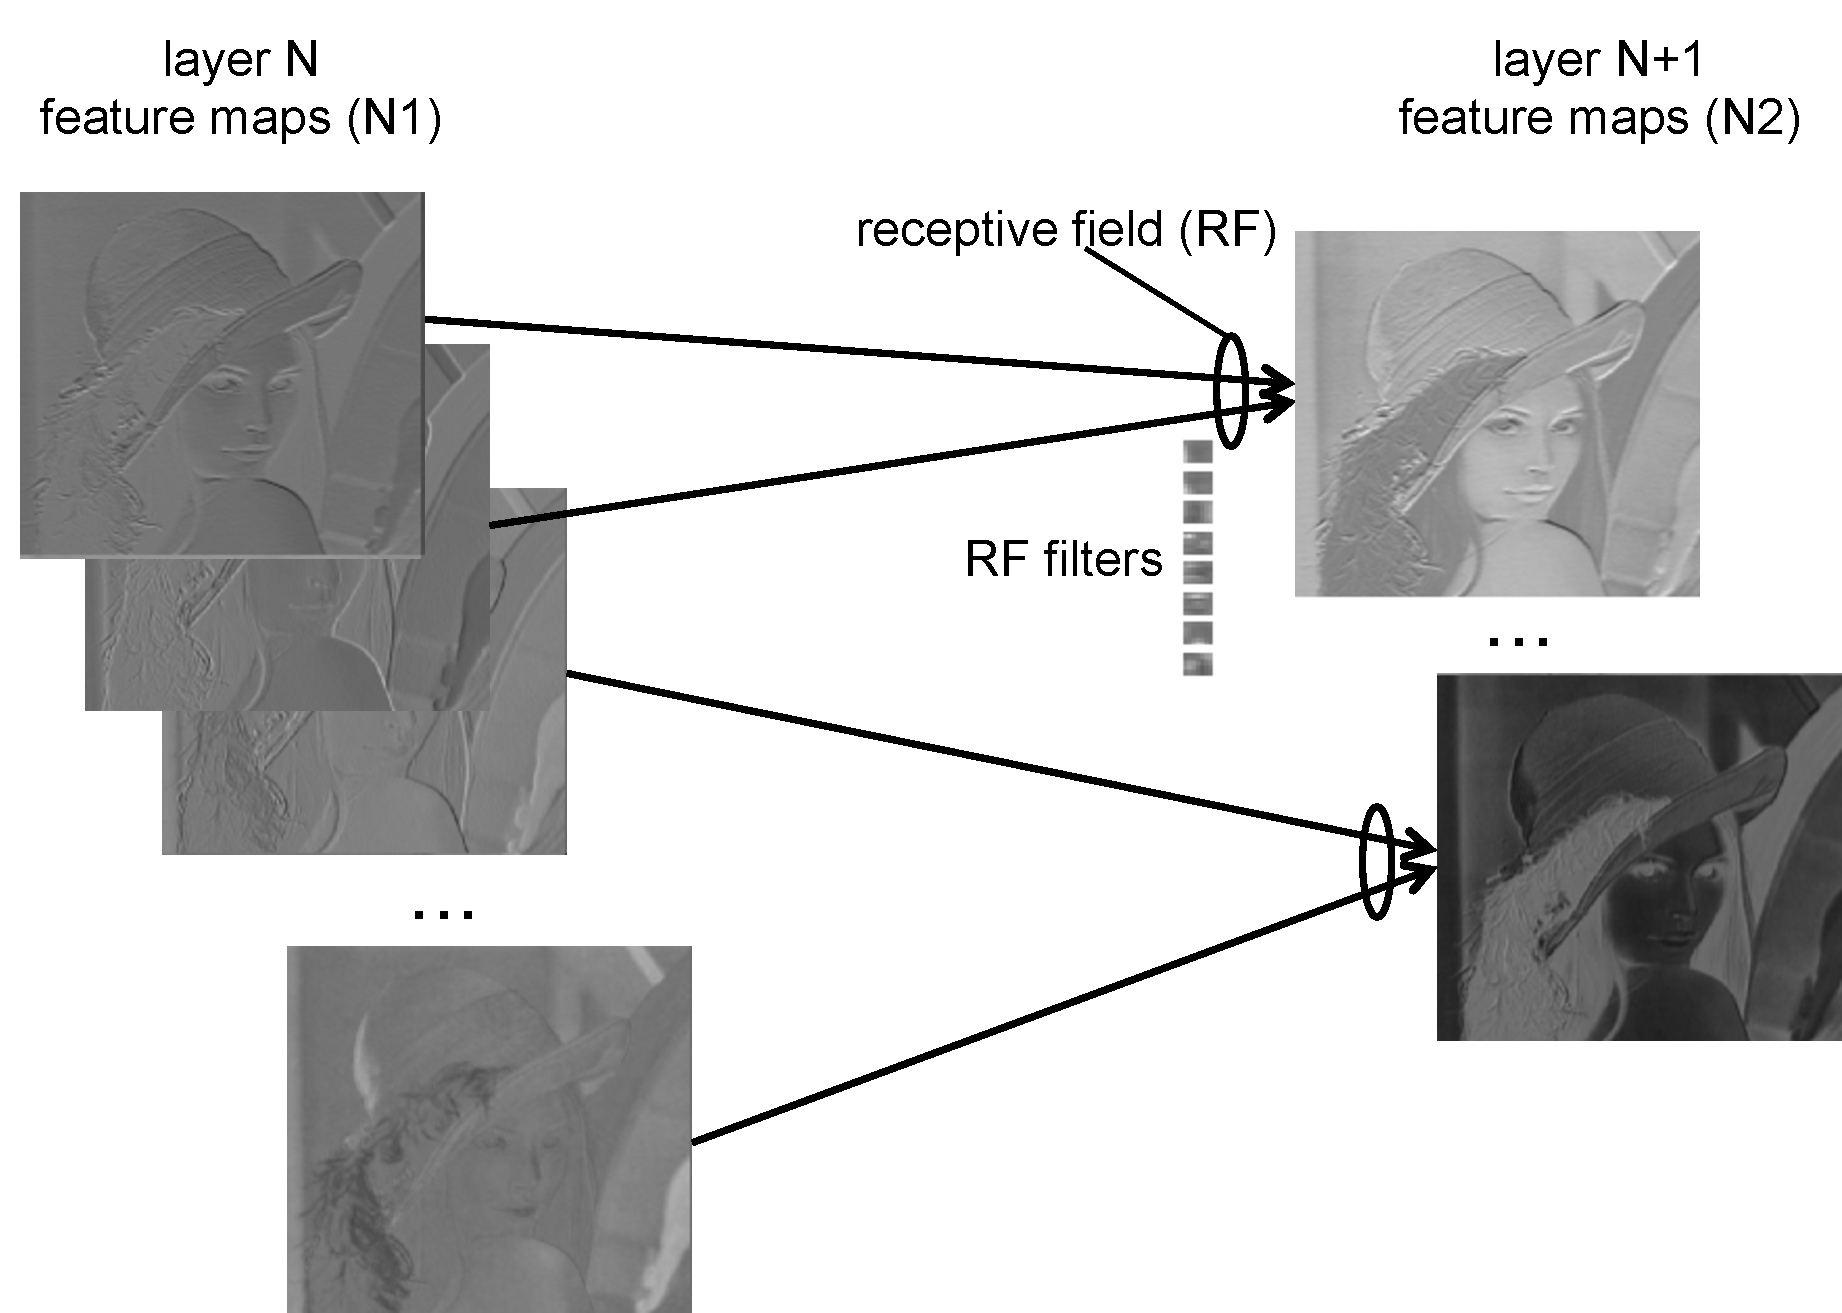
\includegraphics[width=3.5in]{fig-learnlayers.pdf}
\caption{Learn layers}
\label{fig-learnlayers}
\end{wrapfigure}

In the figure we show two layers of a deep network: layer $N$ and layer $N+1$. The maps on the left of the figure, are the $N1$ output feature maps of the $N$-the layer in response to an input image. The maps on the right of the figure, are the $N2$ outputs of the first convolutional module of layer $N+1$. 
Our learning technique groups feature maps from layer $N$ into "receptive fields" (RF). These receptive fields are the input of one or multiple maps in layer $N+1$. We form these RF by grouping a small number "fanin" of layer $N$ features that co-occur in one or multiple sets of feature maps from layer $N$. In other words, we look for features that are highly activated in the same pixel, and we group these features into the RF. The idea behind this step is to group features that occur often together in the data. These RF are then representative of the connections between features of one layer and the next layer, and are completely obtained in a data-driven approach.
In order to learn the filters for layer $N+1$ convolutional module, we perform clustering (Clustering Learning) only within the RF (and not all $N1$ maps). 
We then obtain both a set of connections from layer $N$ to layer $N+1$ and the filters used by layer $N+1$ convolutional module.

The main driving force for this idea is a bio-inspired model of learning in the mammalian brain. It is widely believed that one of the possible physical mechanism of learning in the brain is the Hebbian method \cite{hebbia}. This learning method suggests that a group of pre-synaptic neurons is strongly connected to a post-synaptic neuron if the group (or receptive field, RF) can predict the response of the post-synaptic neuron. In other words neuron in the RF have strong connections to a neuron in layer $N+1$ if they can predict its response. Our idea above implements a real-valued approximation of this learning rule. The RF group features that are highly activated together in the same location. This group of highly activated features will then propagate a high value to the same location in the relative map of layer $N+1$. This implements the Hebbian rule.



There is not much other work in learning connections [cite: adam coates, yi-lan boreau] 


\section{Methods}
\label{sec-methods}


We used the Torch7 software for all our experiments \cite{collobert_torch7_2011}, since this software can reduce training and learning of deep networks by 5-10 times compared to similar Matlab and Python tools.


\subsection{Input data}

We use input color video sequences of people talking in front of a camera as captured from a computer camera. The input video was resized to 120x 80 pixels and was contrast normalized separately on each RGB channel with a 9x9 gaussian filter using the Torch7 "nn.Spatial Contrastive Normalization" function.

We use the XXXX dataset to test how the unsupervised network would perform on labeled data. The XXXXX dataset has a training size of 52,684 32x32 images and a test size of 5,854 32x32 images. The dataset has two classes: 'face' and 'background'. Input data was contrast normalized separately on each RGB channel with a 9x9 gaussian filter using the Torch7 "nn.Spatial Contrastive Normalization" function.

%\begin{figure}
%        \centering
%        \begin{subfigure}[b]{0.5\textwidth}
%                \centering
%                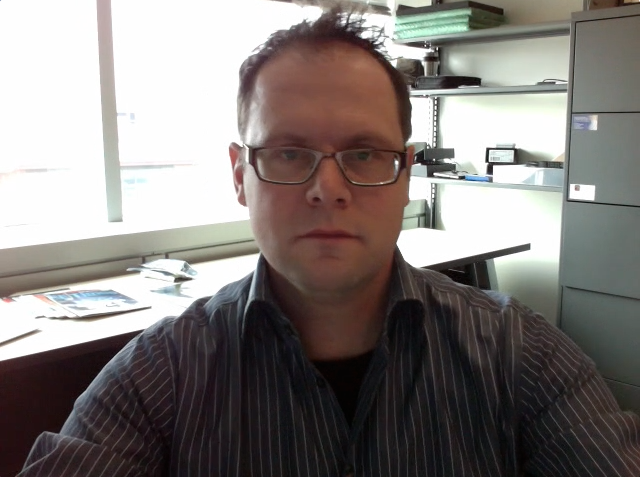
\includegraphics[width=2.65in]{fig-examplevideo.png}
%                \caption{Example frame of the training video sequence.}
%        \end{subfigure}%
%        ~%add desired spacing between images, e. g. ~, \quad, \qquad etc. 
%          %(or a blank line to force the subfigure onto a new line)
%        \begin{subfigure}[b]{0.5\textwidth}
%                \centering
%                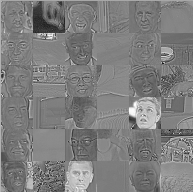
\includegraphics[width=2in]{fig-faceds.png}
%                \caption{Examples from the NYU face dataset.}
%        \end{subfigure}
%        \caption{}
%\end{figure}

Even if other groups showed slight improvements using the YUV color space \cite{jarrett_what_2009}, we did not use it. Rather, we kept the images in their original RGB to keep the model closer to biological human vision, where the retina is broadly sensitive to roughly RGB \cite{wandell_foundations_1995}. 

Also we did not use whitening of data (such as ZCA whitening) even if other groups have shown clear advantages of using it.  We did not use whitening because of two main reasons: first, it is not applicable for general-purpose vision system where an a-priori dataset cannot be obtained. Second, whitening computation is very expensive (similar to the first layer of a convolutional neural network) and we instead replaced it with local contrast normalization, which is a bio-inspired technique to whiten the input data removing its mean bias and adapting the input dynamic range.



\subsection{Network architecture}
\label{sec-net-arch}

We experimented by training an unsupervised deep neural network with 2 layers, not counting pooling and normalization operations. The two layers were composed of a two-dimensional convolutional linear filtering stage, a spatial max pooling stage, and a subtractive and/or divisive normalization layer for removing the mean and resetting the std of all outputs to unity. 
The filters of the first two layers are generated with unsupervised clustering algorithms, as explained below. 
Using the naming convention in \cite{lecun_convolutional_2010}, for each layer $l$  $x_i$ is an input feature map, $y_i$ is an output feature map. The input of each layer is a 3D array with $n_l$ 2D feature maps of size $n_{l1} \cdot n_{l2}$. Each component (pixel, neuron) is denoted $x_{ijk}$. The output is also a 3D array, $y_i$ composed of $m_l$ feature maps of size $m_{l1} \cdot m_{l2}$.

The layers in the clustering learning network used the following sequence of operations:
\begin{enumerate}
\item Volumetric Convolution module (1st layer): performing convolutions on images with the learned volumetric CL filters
\item Spatial Convolution module (2nd layer): performing convolutions on images with the learned CL filters: $yc_i=b_j+\sum_i{k_{ij}\ast x_i}$, where $\ast$ is the 2D discrete convolution operator and $b_j$ is a trainable bias parameter.
\item Spatial Max Pooling module: $yp_i = max_{n \times n}(yc_{ij})$ with $n =  2$ in this work.
\item Hyperbolic tangent nonlinearity: $ynl_i = tanh(yp_i )$
\item Spatial Subtractive or Contrastive Normalization: to zero the data mean, reset std to unity. The subtractive normalization operation for a given site $ynl_{ijk}$ computes: $v_{ijk} = ynl_{ijk} - \sum_{ipq} w_{pq} \cdot ynl_{i,j+p,k+q}$, where $w_{pq}$ is a normalized truncated Gaussian weighting window (typically of size 9x9). The divisive normalization computes $y_{ijk} = v_{ijk}/max(mean(\sigma_{jk}),\sigma_{jk})$ where $\sigma_{jk} = (\sum_{ipq} w_{pq} \cdot v^2_{i,j+p,k+q})^{1/2}$. The local contrast normalization layer is inspired by visual neuroscience models.
\end{enumerate}


All networks used 32 filters on the first layer, 64 filters on the second layer. Clustering learning networks used a fully connected input to 1st, and 1st to 2nd layer. We experimented with SLAC connections \cite{coates2012emergence}. In this case we used 4x more features than the numbers given above as beginning features, and then we decreased them to the same size of 32,64 in each respective layer. After the Convolution modules we added a SpatialMaxMap module to compute the groups and reduce the feature numbers.



\subsection{Learning}
We use k-means clustering algorithm (we refer to this step as \textit{Clustering Learning algorithm}) to learn a set of 32 filters in the first layer, and 64 filters in the second layer. The techniques and scripts are general and can quickly modified to learn any number of filters. The filter sizes on both layers was set to 5 x 5 pixels.






%Larger network:
%This network can be executed in real-time with accelerated hardware [neuflow]



\section{Results}
\label{sec-results}




%\begin{table}[htdp]
%\caption{Network execution time on a 320 x 240 frame.}
%\begin{center}
%\begin{tabular}{|c|c|c|c|c|}
%\hline\hline
%1L filters	& 2L filters	& type				& frames 		&time [ms] \\ 
%\hline
%32 		& 64 			& full					& 1			& 356.50 \\
%32 		& 64 			& full LCN				& 1			& 421.37 \\
%32 		& 64 			& full	 LCN				& 2			& 560.45 \\
%32 		& 64 			& full	 LCN				& 4			& 858.28 \\
%128 $\rightarrow$ 32 	& 64 			& SLAC 1L			& 1			& 654.25 \\
%128 $\rightarrow$ 32 	& 256 $\rightarrow$ 64 	& SLAC 2L			& 1			& 1067 \\	
%64		& 128		& full					& 1			& 1036 \\
%8		& 32			& CNN				& 1			& 6.04 \\
%
%\hline\hline
%\end{tabular}
%\end{center}
%\label{table2}
%\end{table}

Table \ref{table2} reports the execution time of some of the tested networks reported in table \ref{table1}.



\section{Discussion}

We presented results on clustering learning algorithms for general-purpose vision system. These algorithms can be used to train multi-layer feed-forward neural networks from videos in minutes. We show results on ...



%\section{TODO}
%


\subsubsection*{Acknowledgments}
We are especially grateful to the the Torch7 developing team, in particular Ronan Collobert, who first developed this great, easy and efficient tool, Clement Farabet, Koray Kavukcuoglu, Leon Bottou. We could not have done any of this work without standing on these giants shoulders.

\bibliography{clustering}
\bibliographystyle{unsrt}



\end{document}
